\documentclass[12pt]{article}

\newcommand{\CiteMathPackage}{../../math}
\newcommand{\CiteReference}{../reference.bib}

% Packages
\usepackage{setspace,geometry,fancyvrb,rotating}
\usepackage{marginnote,datetime,enumitem}
\usepackage{titlesec,indentfirst}
\usepackage{amsmath,amsfonts,amssymb,amsthm,mathtools}
\usepackage{threeparttable,booktabs,adjustbox}
\usepackage{graphicx,epstopdf,float,soul,subfig}
\usepackage[toc,page]{appendix}
\usdate

% Page Setup
\geometry{scale=0.8}
\titleformat{\paragraph}[runin]{\itshape}{}{}{}[.]
\titlelabel{\thetitle.\;}
\setlength{\parindent}{10pt}
\setlength{\parskip}{10pt}
\usepackage{Alegreya}
\usepackage[T1]{fontenc}

%% Bibliography
\usepackage{natbib,fancybox,url,xcolor}
\definecolor{MyBlue}{rgb}{0,0.2,0.6}
\definecolor{MyRed}{rgb}{0.4,0,0.1}
\definecolor{MyGreen}{rgb}{0,0.4,0}
\definecolor{MyPink}{HTML}{E50379}
\definecolor{MyOrange}{HTML}{FF5733}
\newcommand{\highlightR}[1]{{\emph{\color{MyRed}{#1}}}} 
\newcommand{\highlightB}[1]{{\emph{\color{MyBlue}{#1}}}}
\newcommand{\highlightP}[1]{{\emph{\color{MyPink}{#1}}}}
\newcommand{\highlightO}[1]{{\emph{\color{MyOrange}{#1}}}}
\usepackage[bookmarks=true,bookmarksnumbered=true,colorlinks=true,linkcolor=MyBlue,citecolor=MyRed,filecolor=MyBlue,urlcolor=MyGreen]{hyperref}
\bibliographystyle{econ}

%% Theorem Environment
\theoremstyle{definition}
\newtheorem{assumption}{Assumption}
\newtheorem{definition}{Definition}
\newtheorem{theorem}{Theorem}
\newtheorem{proposition}{Proposition}
\newtheorem{lemma}[theorem]{Lemma}
\newtheorem{example}{Example}
\newtheorem{corollary}[theorem]{Corollary}
\usepackage{mathtools}
\usepackage{\CiteMathPackage}

\begin{document}

%??%??%??%??%??%??%??%??%??%??%??%??%??%??%??%??%??%??%??%??%??%??%??%??%??%??
%?? Title
%??%??%??%??%??%??%??%??%??%??%??%??%??%??%??%??%??%??%??%??%??%??%??%??%??%??

\title{\bf Job Matching within and across Firms, International Economic Review, 2015}
\author{Wenzhi Wang \thanks{This note is written in my MPhil period at the University of Oxford.} } 
\date{\today}
\maketitle

\citet{pastorinoJobMatchingFirms2015}

\section{Introduction}

Over their careers, workers typically advance through a hierarchy of jobs within firms and turn over across firms, experiencing both wage increases and decreases. These two types of job mobility within and across firms have been largely analyzed as distinct phenomena by two virtually separate literatures on so-called \highlightB{internal} and \highlightB{external} labor markets. In this article, I propose a simple unified framework that integrates both dimensions of job dynamics in the presence of uncertainty and learning about workers' ability. I characterize equilibrium assignment and wages for varying degrees of generality of ability across jobs and firms. I also explore how differences in the speed of learning about ability across jobs and firms affect salient features of the dynamics of jobs and wages. The implications of the model are consistent with well-documented features of careers, cast new light on common findings, and explain patterns fo careers previously thought difficult to reconcile with the presence of uncertainty and learning. 

This unified framework addresses a shortcoming of the two literatures mentioned above: Models of job mobility within firms are mostly silent about worker turnover, whereas models of turnover across firms commonly ignore job mobility in firms. By relaxing the assumption that ability is either fully general or fully specific to jobs or firms, the framework proposed can simultaneously explain findings on careers in firms as well as on turnover across firms and occupations. This framework also suggests a new endogenous mechanism of compensating wage differentials for the \highlightP{differential informativeness} of jobs that leads wages to deviate from a worker's (expected) output in an otherwise frictionless environment. \highlightP{This mechanism gives rise to discrete wage increases at promotion in a firm, and discrete wage changes upon turnover across firms, for workers with any level of experience.} Since the ability of experienced workers may be known precisely, this feature of wage dynamics has long been considered hard to explain simply based on job matching and learning about ability. 

\highlightR{Notes: I don't really understand how this mechanism leads to discrete increase in wages.}

Formally, I consider a competitive overlapping generations economy in which a worker's ability (either high or low) is initially unknown to all agents, including that worker. Firms operate technologies that are described by a collection of jobs, which produce output and information. These technologies display complementarity between ability and jobs so that jobs can be ordered by the additional output produced by a worker of high ability relative to a worker of low ability. 

When a worker is employed, a two-sided heterogenous trade in labor services and information takes place. The worker provides labor services to a firm, the perceived quality of which is summarized by the common belief about his ability. The firm provides information to the worker that is indexed by the informativeness of the assigned job. Hence, workers select into jobs, in part, because of the information acquisition possibilities that employment offers. As a result, workers' career paths reflect a gradual process of accumulation of information about their suitability for the jobs in the economy, which leads workers to optimally advance through jobs both within and across firms. 

I study first a simple \highlightB{general ability} model in which ability is general across firms and jobs, and jobs are equally informative about ability. In this case, equilibrium assignment follows a \highlightB{hierarchy rule}: Success leads to promotion to higher-ranked jobs in a firm and possibly turnover to other firms, at which workers are paid higher wages and high-ability workers have greater comparative advantage. Similarly, failure leads to demotion to lower-ranked jobs and possibly turnover to other firms, at which workers are paid lower wages and low-ability workers have greater comparative advantage.

This model captures several observed features of careers in firms. For instance, for individuals continually employed at a firm, wages increase at promotion, real wage decreases are common but demotions are rare, and promotions and wage increases are serially correlated. In addition, when firms differ in their technologies, workers turn over across firms, and their turnover is associated with either wage increases (in the case of successful workers) or wage decreases (in the case of unsuccessful workers). This version of the model also generates a cross-sectional distribution of wages that is positively skewed, as in the data, and more skewed as the chance of failure for young workers increases. Intuitively, when success is difficult to achieve, high wages reward the relatively small proportion of individuals whose ability is perceived to be high. 

In this general ability model, job and wage changes within a firm are mainly generated by the assumption that ability is general across a firm's jobs, whereas turnover and the associated dynamics of wages follow from the assumption that ability is general across firms. Some evidence challenges this latter assumption. 

Motivated by this evidence, I consider a \highlightB{firm-specific} version of the model in which a worker's ability is specific to firms but general across a firm's jobs. A novel implication of this model is that equilibrium job assignment has now a two-part form. First, for each firm, a modified Gittins index is computed, and a worker is assigned to the firm with the highest value of such index. Second, given the assigned firm based on this index, the assigned job within the firm follows a within-firm hierarchy rule. Success in a given firm increases the index of that firm only, whereas failure lowers it. Hence, continual success leads workers to move up the hierarchy of jobs of a firm but remain continuously employed at a same firm. Continual failure, instead, leads to demotion within a given firm until the modified Gittins index of the firm drops below that of the next-best firm, in which case a worker turns over to the next-best firm. Thus, by retaining the assumption that ability is general across a firm's jobs, the model still generates the key features of careers in firms reproduced by the general ability model. By allowing ability to be specific to firms, the model also gives rise to a declining hazard of separation with tenure in a firm and positive returns to tenure. 

More recent empirical evidence suggests that ability may be specific to occupations instead of firms. Based on this evidence, I also analyze an \highlightB{occupation-specific} version of the model, in which a worker's ability is specific to occupations, interpreted as collections of jobs with similar skill requirements, and each firm has a collection of jobs of possibly different occupations. In this case, equilibrium assignment follows a modified Gittins index rule for occupational choice and a hierarchy rule for job assignment within each occupation. This version of the model gives rise to a hazard of occupational switching that eventually decreases with tenure in an occupation and experience in the labor market as well as returns to tenure in occupation. This model also matches the observation that the relatively low and high wage earners in an occupation have the highest probability of leaving it. 

Altough the framework proposed reproduces salient features of careers by allowing for varying degrees of generality of ability across jobs and firms, one important aspect of the data is known to be difficult to reconcile with learning models of careers. In firms, wage increases at promotion tend to rise with the level of a job in a firm's hierarchy of positions, and so they are also larger for workers with more tenure and labor market experience, typically assigned to higher levels. Models that assume jobs are equally informative about ability are partly at odds with this feature of the data. The reason is that after a number of periods of observation of a worker's output, a worker's ability should be fairly well known. Then additional output observations on workers with greater tenure and labor market experience should have a small impact on the market expectation about their ability and, thus, on their wages, leading to progressively smaller wage increases at promotion. 

To address this limtation, I consider a \highlightB{differential learning} version of the model in which jobs differ in informativeness, that is, in the information about ability that job performance conveys. I show that the resulting different speed of learning across jobs gives rise to compensating wage differentials across jobs for their different informativeness. This mechanism can naturally account for the pattern of wage increases at promotion just discussed. Intuitively, when higher-level jobs in a firm's hierarchy are less informative about ability than lower-level ones, each promotion compensates a worker for the loss in information associated with the new assignment. As a result, wage premia in the form of discontinuous increases in wages accrue upon promotion from a \highlightP{more} informative job to a \highlightP{less} informative one to compensate a worker for the lost information. In this case, equilibrium assignment is no longer solely dictated by the static comparative advantage of workers across jobs. Rather, the trade-off between output and information implied by job assignment leads workers to be assigned to jobs at which they have a static comparative disadvantage but to be dynamically compensated for the associated current loss in wages with the greater information that these jobs provide as well as with wage premia at promotion.

\section{The Economy}

\subsection{Setup}

Consider a market in which $N$ firms compete for workers in each period of an infinite (or finite) horizon, with dates $t \geq 1$. All firms and workers share a common discount factor, $\d \in [0, 1)$. In the economy, one good is produced and consumed, the price of which is normalized to one. A worker's talent or productive ability at each firm $f$ is described by the skill type $s \in \bc{a, b}$, which is assumed to be unobserved by firms and workers -- including the given worker. I refer to a worker of type $a$ as a high-ability worker and a worker of type $b$ as a low-ability worker; later, I consider the case in which ability is described by a vector of skill types. Each worker inelastically supplies one unit of labor each period. At $t=1$, the information available about a worker's skill type is summarized by the prior probability $p_1$ that the worker is of high ability. I assume that there is a continuum of workers with measure one. I elaborate on the structure of the population in the economy in the next section. 

Each firm is endowed with a production set that consists of $K_f$ tasks or jobs. A worker's output in a period is stochastic, and its distribution depends on the worker's ability, the employing firm, and the assigned job. The output produced in period $t$, when the worker is employed at job $k$ of firm $f$, $1 \leq k \leq K_f$, is denoted by $y_{fk} \in \bc{y_{fHk}, y_{fLk}}$, with $y_{fHk} > y_{fLk} > 0$. The probability of high output at job $k$ of firm $f$ is $\a_{fk}$ for a worker of ability $a$ and $\b_{fk}$ for a worker of ability $b$, with $0< \b_{fk} < \a_{fk} < 1$. Thus, a job is a four-tuple $\bp{\t_{fk}, y_{fHk}, y_{fLk}}$, where $\t_{fk} = \bp{\a_{fk}, \b_{fk}}$ records the \highlightB{informativeness} of the job. Depending on how these job parameters vary across jobs and firms, the productivity of a worker of a given ability correspondingly varies. I assume that a worker's output, or performance, is symmetrically observed by all firms and workers, and denote by $p_t$ the prior probability that firms and workers assign to a worker being of high ability at the beginning of period $t$ or, in short, the \highlightB{prior} at the beginning of period $t$. Since $\a_{fk} > \b_{fk}$, observing high output, $y_{fHk}$, in any period at the job of any firm increases $p_t$. 

At the beginning of period $t \geq 1$, the one-period expected output of a worker assigned to job $k$ of firm $f$, conditional on his ability being high and low, respectively, is 
\begin{equation}
    \label{1}
    \ol{y}_f\of{a, k} = \a_{fk} y_{fHk} + \bp{1-\a_{fk}}y_{fLk}, \quad \ol{y}_f\of{b, k} = \b_{fk} y_{fHk} + \bp{1-\b_{fk}}y_{fLk}.
\end{equation}
Given $p_t$, the one-period expected output $y_f\of{p_t, k}$ of a worker at job $k$ of firm $f$ in $t \geq 1$, averaged over the two skill types of the worker, is affine in the prior $p_t$ and given by 
\begin{equation}
    \label{2}
    y_f\of{p_t, k} = p_t \ol{y}_f\of{a, k} + \bp{1 - p_t} \ol{y}_f\of{b k} = c_{fk} + d_{fk} p_t,
\end{equation}
with $c_{fk} = \ol{y}_f\of{b, k}$ and $d_{fk} = \ol{y}_f\of{a, k} - \ol{y}_f\of{b, k}$. Note that $f$ and $k$ in $y_f\of{p_t, k}$ simply index $\bp{\t_{fk}, y_{fHk}, y_{fLk}}$ so that $y_f\of{p_t, k}$ is shorthand for $y\of{p_t, \t_{fk}, y_{fHk}, y_{fLk}}$. 

The assumptions that $y_{fHk} > y_{fLk}$ and $\a_{fk} > \b_{fk}$ imply that a high-ability worker has an \highlightP{absolute advantage} at all jobs. Hence, expected output, $y_f\of{p_t, k}$, increases with $p_t$. This pattern of absolute advantage implies that in equilibrium, wages increases after high output but decrease after low output in a job, as often observed. I also assume \highlightP{complementarity} between ability and jobs in that 
\begin{equation}
    \label{3}
    \ol{y}_f\of{a, k+1} \geq \ol{y}_f\of{a, k}, \quad \ol{y}_f\of{b, k} \geq \ol{y}_f\of{b, k+1}, \quad k = 1, \ldots, K_f - 1.
\end{equation}
Figure \ref{fig-1} illustrates this assumption for three jobs. \highlightO{High-ability workers (ability $a$) have the highest expected output in job 3, the next highest in job 2, and the lowest in job 1, whereas low-ability workers (ability $b$) display the opposite pattern.} By assumption (\ref{3}), high-ability workers have a \highlightP{comparative advantage} at higher-index jobs. To interpret this assumption, imagine raking jobs by their complementarity with ability, which reflects, for instance, the complexity of their tasks, from least (job 1) to most complementary (job $K_f$). Then, higher-indexed jobs are those involving more complex tasks whose complementarity with ability is more pronounced. This pattern of comparative advantage leads successful individuals to advance over time to higher-indexed jobs of a firm's hierarchy, as consistent with the data.
\begin{figure}[H]
	\noindent\caption{Benchmark assignment rule and wages with equally informative jobs}
	\centerline{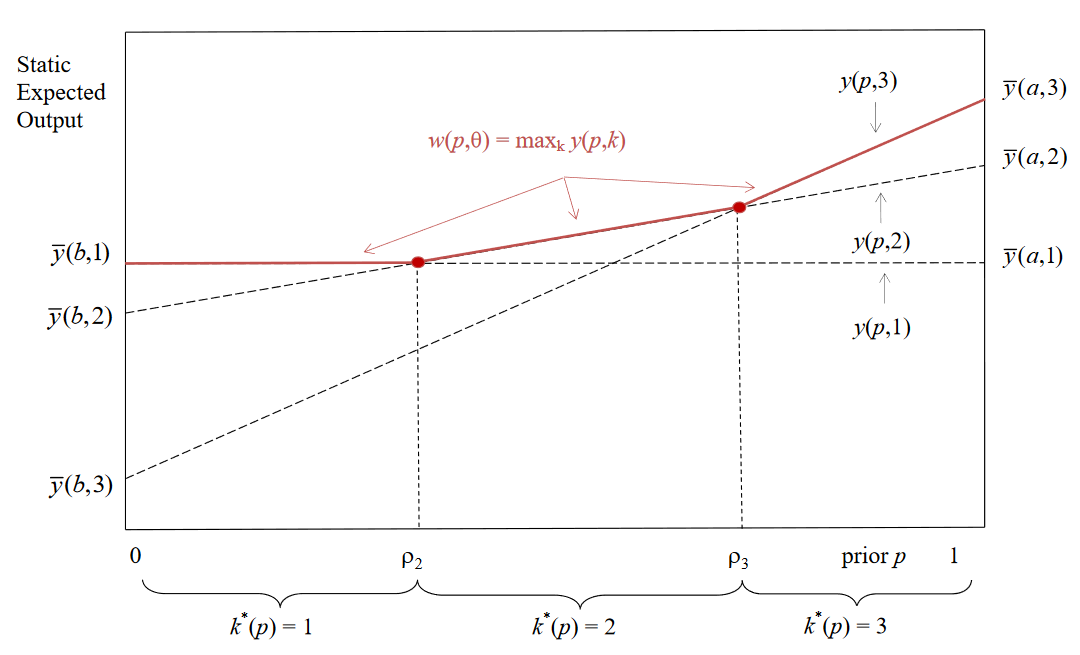
\includegraphics[scale=0.8]{fig-1.png}}
	\label{fig-1}
\end{figure}

For intuition, consider an economy with two jobs: job 1, a mailroom job, and job 2, an executive job. Assumption (\ref{3}) captures the idea that expected output in the mailroom job is relatively insensitive to ability: A low-ability worker produces only slightly less output than a high-ability worker. On the contrary, expected output in the executive job is very sensitive to ability: A low-ability worker produces much less output as an executive compared with a high-ability worker. So, a high-ability worker has a comparative advantage as an executive as well as an absolute advantage in both jobs.

\subsection{Information}

Priors about ability are updated using Bayes' rule: If a worker with prior $p_t$ is assigned to job $k$ to firm $f$, then the updated prior $p_{t+1}$ after a success, $y_{fHk}$, and a failure, $y_{fLk}$, is 
\begin{equation}
    \label{4}
    P_H\of{p_t, \t_{fk}} = \frac{\a_{fk}p_t}{\a_{fk}p_t + \b_{fk}\bp{1-p_t}}, \quad P_L\of{p_t, \t_{fk}} = \frac{\bp{1 - \a_{fk}}p_t}{\bp{1 - \a_{fk}}p_t + \bp{1 - \b_{fk}}\bp{1-p_t}}.
\end{equation}
Job $k$ of firm $f$ is said to be \highlightB{more informative} than job $k^\prime$ of firm $f^\prime$ if 
\begin{equation}
    \label{5}
    P_H\of{p_t, \t_{fk}} \geq P_H\of{p_t, \t_{f^\prime k^\prime}}, \quad P_L\of{p_t, \t_{fk}} \leq P_L\of{p_t, \t_{f^\prime k^\prime}},
\end{equation}
that is, the posterior reached after output is realized at job $k$ is a mean-preserving spread of the posterior reached after output is realized at job $k^\prime$. I model the distribution of output at each job as possibly asymmetric across skill types in that $\b_{fk}$ need not equal $1 - \a_{fk}$. With symmetric and identically distributed signals at all jobs, that is, with $\b_{fk} = \b = 1 - \a = 1 - \a_{fk}$, it follows that $P_H\of{P_L\of{p_t, \t_{fk}}, \t_{fk}} = P_L\of{P_H\of{p_t, \t_{fk}}, \t_{fk}} = p_t$, so one failure exactly offsets one success. In this case, if a worker is promoted from job $k$ to $k+1$ after a success, then that worker is necessarily demoted to job $k$ after a failure in job $k+1$. Asymmetric signals, instead, allow for more flexible patterns of promotion and demotion. For example, consider an extreme case in which $\a=1$ and $\b$ is close to 1, so that high-ability workers never fail and low-ability workers rarely fail. In this case, a success is not very informative about ability, so promotions are gradual, occurring only after sufficiently many successes, since no single success perfectly reveals ability. Demotions, instead, are rare, since the probability of failure for both worker types is small. This combination of gradual, frequent promotions and rare demotions is commonly observed in the data. 

The discrete Bernoulli structure assumed here also allows for a flexible time profile of the variance of posterior beliefs about a worker's ability and thus job assignment wages. \footnote{In contrast, a worker's output is often modelled as normally distributed in the literature. Coupled with normally distributed priors, this assumptions implies that variance of posterior beliefs about a worker's ability declines deterministically with the number of signals observed, that is, with tenure or with tenure and experience. Hence, the learning component of these models predicts that the longitudinal variance of wages for a single worker should also decline deterministically with tenure or experience, which is not universally observed.} In practice, individual performance evaluations, normally interpreted as proxies for output signals, are recorded based on coarse classification scales. It is easy to show that if performance evaluations are discrete, then assuming discrete signals entails no loss of generality. Hence, modelling output signals as discrete is both conceptually and empirically appealing. 

\section{A Competitive Equilibrium}

Each worker alive in period $t$ faces a constant probability of dying of $1 - \g$ with $\g \in \bp{0, 1}$. At time $t$ the probability of being alive at $t+s$ is thus $\g^s$. In each period, a measure $1-\g$ of workers are born with an initial distribution of priors about ability denoted by $G\of{p_1}$. Using the law of large numbers, the measure of any given cohort of workers declines deterministically with time at rate $1-\g$. Using $n_{ts}$ to denote the measure in period $s$ of a cohort born in period $t$, it follows that $n_{ts} = \bp{1-\g}\g^{s-t}$. The measure of the total population of workers in period $s$ is $n_s = \sum_{t=-\infty}^s n_{ts}$, which is constant and equal to 1. 

I assume there exist perfect annuity markets, in which firms make annuity payments to workers when annuity payments to workers when they are alive and inherit their wealth when they die, and complete insurance markets against the idiosyncratic risk of success or failure in a job. 

At birth, workers differ in their initial prior $p_1$ that they are of high ability. Hence, workers' consumption paths are indexed by $p_1$. If $\wt{\d}$ denotes a worker's discount factor, ignoring the possibility of death, then a worker's effective discount factor is $\d = \wt{\d}\g$. A worker born at time $t$ with initial prior $p_1$ has utility given by $\bp{1-\d} \sum_{s=t}^{\infty}\d^{s-t}u\of{c_{ts}\of{p_1}}$, where $c_{ts}\of{p_1}$ is the consumption of a worker of cohort $t$ in period $s$ and the period utility function $u\of{\cdot}$ is concave. 

Consider a stationary equilibrium for this economy. In such an equilibrium, the intertemporal price of goods is constant in calendar time. In particular, the price of goods at time $s$ in units of goods at time $t$ is $1/R^{s-t}$ with $R = 1/\d$. Since there s no aggregate uncertainty in the economy, the combination of annuity markets and insurance markets lets consumers perfectly insure consumption risk. Hence, a worker's budget constraint in a stationary equilibrium is $\sum_{s=t}^{\infty}\d^{s-t} c_{ts} = W\of{p_1}$, where $W\of{p_1}$ is the expected present discounted value of the worker's wages using the market interest rate $R$ in units of the consumption good at date $t$. A worker's problem then conveniently separates into two parts: an \highlightB{intertemporal consumption} problem and a \highlightB{job choice} problem. The optimal path of consumption satisfies $\d^{s-t} u^\prime\of{c_{ts}\of{p_1}}/u^\prime\of{c_{tt}\of{p_1}} = 1/R^{s-t}$, which implies full consumption smoothing in that $c_{ts}\of{p_1} = c_{tt}\of{p_1}$ for all $s$ and $t$. A worker's job choice problem consists of choosing a sequence of jobs so as to maximize the expected present discounted value of wages $W\of{p_1}$, with wages discounted at the market rate $R = 1/\d$.

Consider how wages are determined. When a worker supplies labor to a firm in a given job, a two-sided heterogenous trade in labor services and information takes place. Heterogeneity in labor service arises from workers differing in their unobserved skill types and is summarized by the prior $p$, which may be thought of as a worker's \highlightB{information capital} at date $t$. Thus, a worker with prior $p^\prime$ supplies a labor input that is different from that of a worker with prior $p^{\prime\prime}$. Heterogeneity in information arises from each job supplying a possibly different increment to this information capital. Specifically, in the economy there are $\ol{K} = \sum_f K_f$ jobs and thus at most $\ol{K}$ levels of informativeness. Let $I$ with $I \leq \ol{K}$ denote the number of distinct informativeness levels of the $\ol{K}$ jobs, and let $\T = \bc{\t_1, \ldots, \t_I}$ denote the set of informativeness levels. The commodities exchanged in the labor market, labor input and information, are indexed by $\bp{p, \t}$. Think of there being a market for each such pair: In market $\bp{p, \t}$, the wage in a stationary equilibrium is $w\of{p, \t}$. If a worker is employed in market $\bp{p, \t}$, then the worker receives the wage $w\of{p, \t}$ today, and the worker's information capital is (stochastically) augmented according to (\ref{4}) with $\t_{fk} = \t$. The belief updating rules in (\ref{4}) can be interpreted as production functions of information that a firm supplies to a worker by hiring him.

Given the wage function $w\of{p, \t}$, a worker with prior $p$ must then choose in which of the $I$ \highlightB{information} markets indexed by $\t$ to supply one unit of labor services of type $p$, by solving 
\begin{equation}
    \label{6}
    V\of{p} = \max_{\wt{d}\of{\t}} \sum_{\t \in \T} \wt{d}\of{\t} \bs{\bp{1 - \d}w\of{p, \t} + \d EV\of{p^\prime \mid p, \t}},
\end{equation}
where $EV\of{p^\prime \mid p, \t} = r\of{p, \t} V\of{P_H\of{p, \t}} + \bs{1-r\of{p, \t}} V\of{P_L\of{p, \t}}$ is the worker's expected continuation value, given the prior $p$ and the informativeness level $\t = \bp{\a, \b}$, and $r\of{p, \t} = \a p + \b\bp{1-p}$ is the probability of high output at a job with informativeness $\t$. Note that $\wt{d}\of{\t} = 1$ at some $\t$ and $\wt{d}\of{\t} = 0$ at all others. Then, the optimal decision rule can be written as $d\of{p, \t}$, where $d\of{p, \t} = 1$ when the worker supplies one unit of labor in the market with informativeness level $\t$ and $d\of{p, \t} = 0$ otherwise. 

By (\ref{6}), when choosing a job, a worker with prior $p$ does not simply select the information market with the highest current wage, $w\of{p, \t}$. Rather, in choosing between information markets $\t$ and $\t^\prime$, a worker with prior $p$ balances the difference in current wage, $w\of{p, \t} - w\of{p, \t^\prime}$, against the value of the corresponding difference in information, $EV\of{p^\prime \mid p, \t} - EV\of{p^\prime \mid p, \t^\prime}$. Thus, a worker may choose a market in which current wages are lower than in another because in the chosen market, more information can be acquired, so the worker can achieve a higher expected value of future wages. 

Consider the problem of the representative firm $f$ that takes the wage function $w\of{p, \t}$ as given. Since the firm rents labor services each period, there are no state variables for the firm, and the firm's problem simply reduces to a sequence of static problems. In turn, each static problem reduces to a job-by-job problem for workers of each level of information capital $p$, 
\begin{equation}
    \label{7}
    \max_{l_{fk}} \bs{y\of{p, \t_{fk}, y_{fHk}, y_{fLk}} - w\of{p, \t_{fk}}} l_{fk},
\end{equation}
where $w\of{p, \t}$ is the wage that firm $f$ must pay at any job $k$ with informativeness level $\t_{fk} = \t$ in its production set. The solution $l_{fk}\of{p, \t_{fk}}$ denotes the labor demand of firm $f$ for workers with priors $p$ at job $k$. Notice that since the firm hires a measure of workers and uncertainty about a worker's production is purely idiosyncratic, the law of large numbers implies no uncertainty at the firm level. 

In a stationary equilibrium, the initial distribution $G\of{p_1}$ of priors over newborn workers leads to a time-invariant distribution over all workers, $H\of{p}$. To define this invariant distribution, note that given any possibly noninvariant distribution $H_t\of{p}$, the decision rules of workers about labor supply imply a transition law from $H_t\of{p}$ to $H_{t+1}\of{p}$ of the form $H_{t+1}\of{\cdot} = \G\of{H_t\of{\cdot}, d_t}$, where $d_t$ records the acceptance decisions of all workers in $t$. In a stationary equilibrium, this distribution reproduces itself in that $H\of{p} = \G\of{H\of{p}, d}$ at each $p$. The labor market clearing condition, given a distribution of priors $H\of{p}$ across all workers, can be written at each $\wt{p} \in \bs{0, 1}$ and for each $\t$ as 
\begin{equation}
    \label{8}
    \int_0^{\wt{p}} d\of{p, \t} dH\of{p} = \int_o^{\wt{p}} \sum_{\bc{f, k \mid \t_{fk}=\t}} l_{fk}\of{p, \t_{fk}} dp. 
\end{equation}







\bibliography{\CiteReference}
\end{document}
